% $Id: template.tex 11 2007-04-03 22:25:53Z jpeltier $

% \documentclass{vgtc}                          % final (conference style)
\documentclass[review]{vgtc}                 % review
%\documentclass[widereview]{vgtc}             % wide-spaced review
%\documentclass[preprint]{vgtc}               % preprint
%\documentclass[electronic]{vgtc}             % electronic version

%% Uncomment one of the lines above depending on where your paper is
%% in the conference process. ``review'' and ``widereview'' are for review
%% submission, ``preprint'' is for pre-publication, and the final version
%% doesn't use a specific qualifier. Further, ``electronic'' includes
%% hyperreferences for more convenient online viewing.

%% Please use one of the ``review'' options in combination with the
%% assigned online id (see below) ONLY if your paper uses a double blind
%% review process. Some conferences, like IEEE Vis and InfoVis, have NOT
%% in the past.

%% Figures should be in CMYK or Grey scale format, otherwise, colour 
%% shifting may occur during the printing process.

%% These few lines make a distinction between latex and pdflatex calls and they
%% bring in essential packages for graphics and font handling.
%% Note that due to the \DeclareGraphicsExtensions{} call it is no longer necessary
%% to provide the the path and extension of a graphics file:
%% \includegraphics{diamondrule} is completely sufficient.
%%
\ifpdf%                                % if we use pdflatex
  \pdfoutput=1\relax                   % create PDFs from pdfLaTeX
  \pdfcompresslevel=9                  % PDF Compression
  \pdfoptionpdfminorversion=7          % create PDF 1.7
  \ExecuteOptions{pdftex}
  \usepackage{graphicx}                % allow us to embed graphics files
  \DeclareGraphicsExtensions{.pdf,.png,.jpg,.jpeg} % for pdflatex we expect .pdf, .png, or .jpg files
\else%                                 % else we use pure latex
  \ExecuteOptions{dvips}
  \usepackage{graphicx}                % allow us to embed graphics files
  \DeclareGraphicsExtensions{.eps}     % for pure latex we expect eps files
\fi%

%% it is recomended to use ``\autoref{sec:bla}'' instead of ``Fig.~\ref{sec:bla}''
\graphicspath{{figures/}{pictures/}{images/}{./}} % where to search for the images

\usepackage{microtype}                 % use micro-typography (slightly more compact, better to read)
\PassOptionsToPackage{warn}{textcomp}  % to address font issues with \textrightarrow
\usepackage{textcomp}                  % use better special symbols
\usepackage{mathptmx}                  % use matching math font
\usepackage{times}                     % we use Times as the main font
\renewcommand*\ttdefault{txtt}         % a nicer typewriter font
\usepackage{cite}                      % needed to automatically sort the references
\usepackage{tabu}                      % only used for the table example
\usepackage{booktabs}                  % only used for the table example
%% We encourage the use of mathptmx for consistent usage of times font
%% throughout the proceedings. However, if you encounter conflicts
%% with other math-related packages, you may want to disable it.


%% If you are submitting a paper to a conference for review with a double
%% blind reviewing process, please replace the value ``0'' below with your
%% OnlineID. Otherwise, you may safely leave it at ``0''.
\onlineid{0}

%% declare the category of your paper, only shown in review mode
\vgtccategory{Research}

%% allow for this line if you want the electronic option to work properly
\vgtcinsertpkg

%% In preprint mode you may define your own headline.
%\preprinttext{To appear in an IEEE VGTC sponsored conference.}

%% Paper title.

\title{LLMEval}

%% This is how authors are specified in the conference style

%% Author and Affiliation (single author).
%%\author{Roy G. Biv\thanks{e-mail: roy.g.biv@aol.com}}
%%\affiliation{\scriptsize Allied Widgets Research}

%% Author and Affiliation (multiple authors with single affiliations).
%%\author{Roy G. Biv\thanks{e-mail: roy.g.biv@aol.com} %
%%\and Ed Grimley\thanks{e-mail:ed.grimley@aol.com} %
%%\and Martha Stewart\thanks{e-mail:martha.stewart@marthastewart.com}}
%%\affiliation{\scriptsize Martha Stewart Enterprises \\ Microsoft Research}

%% Author and Affiliation (multiple authors with multiple affiliations)
% \author{Roy G. Biv\thanks{e-mail: roy.g.biv@aol.com}\\ %
%         \scriptsize Starbucks Research %
% \and Ed Grimley\thanks{e-mail:ed.grimley@aol.com}\\ %
%      \scriptsize Grimley Widgets, Inc. %
% \and Martha Stewart\thanks{e-mail:martha.stewart@marthastewart.com}\\ %
%      \parbox{1.4in}{\scriptsize \centering Martha Stewart Enterprises \\ Microsoft Research}}

%% A teaser figure can be included as follows, but is not recommended since
%% the space is now taken up by a full width abstract.
%\teaser{
%  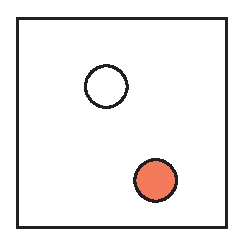
\includegraphics[width=1.5in]{sample.eps}
%  \caption{Lookit! Lookit!}
%}

%% Abstract section.
\abstract{} % end of abstract

%% ACM Computing Classification System (CCS). 
%% See <http://www.acm.org/class/1998/> for details.
%% The ``\CCScat'' command takes four arguments.

% \CCScatlist{ 
%   \CCScat{K.6.1}{Management of Computing and Information Systems}%
% {Project and People Management}{Life Cycle};
%   \CCScat{K.7.m}{The Computing Profession}{Miscellaneous}{Ethics}
% }

%% Copyright space is enabled by default as required by guidelines.
%% It is disabled by the 'review' option or via the following command:
% \nocopyrightspace

%%%%%%%%%%%%%%%%%%%%%%%%%%%%%%%%%%%%%%%%%%%%%%%%%%%%%%%%%%%%%%%%
%%%%%%%%%%%%%%%%%%%%%% START OF THE PAPER %%%%%%%%%%%%%%%%%%%%%%
%%%%%%%%%%%%%%%%%%%%%%%%%%%%%%%%%%%%%%%%%%%%%%%%%%%%%%%%%%%%%%%%%

\begin{document}

%% The ``\maketitle'' command must be the first command after the
%% ``\begin{document}'' command. It prepares and prints the title block.

%% the only exception to this rule is the \firstsection command

\maketitle
\section{Introduction}
Text summarization is an extensively studied NLP task that has many downstream applications.
The recent success of Large Language Models (LLMs) opens up even more application scenarios.
With LLMs, a summarization can be easily generated with zero-shot or few-shot prompting.
Prompt-based summarization provides opportunities for injecting user intent into the summarization process and is therefore highly customizable.
Moreover, prompt-based summarization needs zero or few examples, further allowing users to craft examples tailored to their application contexts.
Each prompt template can thus be seen as a summarization system that demonstrates better capability over previous neural models that do not respond to user intents and require a large amount of labeled data to train. 
The development of such prompt-based summarization systems has become a highly iterative process.

However, the evaluation of prompt-based summarization systems remains a challenge.
The most common approach for evaluating summarization systems is to compare the average score of a computational metric such as ROGUE~\cite{lin2004rouge} on a labeled dataset, but such an approach has been criticized in many ways~\cite{deutsch2022re, bhandari2020re, peyrard2017learning, novikova2017we, durmus2020feqa} even in previous neural-based summarization systems.
Evaluating LLM summarization systems using computational metrics is even more questionable.
First, computational metrics do not reliably quantify system improvements among state-of-the-art systems because they do not distinguish high-quality summaries very well~\cite{deutsch2022re, bhandari2020re, novikova2017we}.
Much of the improvements observed over such metrics between a newly proposed system and the baseline system are attributed to successfully distinguishing the `easy' cases, i.e.cases where the baseline system fails very badly.
LLMs have been demonstrated to be able to produce human-level summaries that the quality differences are too nuanced for computational metrics to capture~\cite{zhou2022large}.
Second, computational metrics rely on reference texts (ground-truths) to compute, which are often crafted by human writers.
Such reference texts are expensive to craft and do not generalize well across domains. 
The usage of such reference texts also limits the customizability of LLMs.
More recently, reference-free metrics such as $Q^2$~\cite{honovich2021q2} or FEQA~\cite{durmus2020feqa} have been proposed for evaluation without reference texts.
% The rationale behind these approaches is that a question should have similar answers from the input text and the summarized text.
However, they are reported to be capturing spurious correlations~\cite{durmus2022spurious}.
Another trend of reference-free evaluation is using LLM as evaluators, but they do not yet exhibit a consistent correlation with human judgment~\cite{zhou2022large}.
In addition, all these metrics have a high computation time that is not suitable for an iterative development process.

One commonality among the above approaches is that they are all automatic approaches that completely exclude humans in the evaluation process.
We argue that the capability of LLMs in summarization has reached, if not exceeded, the human level.
Prompt-based summarization can be applied to almost any application scenario, with a high level of customizability.
The quality of a summarization system in real-world scenarios is arguably too complex to be quantified by computational metrics.
Consequently, the evaluation of such summarization systems will likely be incomprehensive without a human in the loop.

In addition, embedding analysis has been shown to be effective in explaining LLM behaviors such as document relevancy ranking~\cite{lucchese2023can, mishra2023promptaid}.
Following this direction, we propose to evaluate summarization systems by analyzing the embedding distribution of the input text and summarized text.
We present experiments to show that the summarization system is essentially a transformation function that maps the input text embeddings to summarized text embeddings.
Thus, the quality of a summarization system can be evaluated by analyzing the embedding distribution of the input text and summarized text.

Following the above discussion, we propose a visual analytic system that incorporates a human-in-the-loop approach to evaluate a summarization system.
Our system provides a visualization of the embedding distribution of the input text and summarized text and interactions to analyze the distributions.
In addition to the distribution visualization, we further incorporate existing computational metrics in the system as complementary signals.
Our contributions are as follows:
\begin{itemize}
   \item We show that embedding analysis is a promising approach for evaluating summarization systems.
   \item We propose to evaluate summarization systems in a human-in-the-loop approach and develop a visual analytic system to support embedding analysis for summarization system evaluation.
   \item We evaluate our system with quantitative experiments and qualitative expert reviews.
\end{itemize}


\section{Related Works}
\subsection{Summarization Metrics and Meta Evaluation}
\paragraph{Computational Metrics}
\paragraph{Reference-free Metrics}
\paragraph{LLM evaluator Metrics}

Outline
1. Existing problems with using automatic summarization metrics to guide prompt optimization/evaluate prompts:
    - LLM produces human-level summaries that quality differences are too nuanced for automatic metrics to capture [5]
    - Correlation with human judgment is questionable [6]
    - A trade-off between abstractive and faithfulness must be made for automatic metrics [10]
    - automatic metrics tend to correlate well with humans at the system level but have poor correlations at the instance level [2, 3]
    - No single metric can outperform (correlation) across datasets -> This suggests different datasets need to use different metrics [2]
    - Metrics can not reliably quantify improvements if the difference is too small -- much success is attributed to ranking `easy' cases [1, 2, 6]

2. Problems with LLM evaluators: outperforms automatic metrics, but do not exhibit consistent correlation with human judgment [5]
3. Problems with reference-free metrics: capturing spurious correlation (highly correlated with spurious metrics like text length, word overlap, and perplexity) [8]
4. LLM evaluators and reference-free metrics have higher computation time
5. New problem in summarization task when LLM is used: Robustness

Notes:
    1. LLM benchmarks are neither informative nor actionable for application developers
    2. evaluation of a new metric: system-level vs. instance level: which one would visual metric succeed at?
    3. reference-based metrics are not able to capture factuality (faithfulness) errors [7]
    4. Meaningful -> Grammatical/Readable/Formal -> Faithful -> Capturing gist


\subsection{Latent Space Visualization}

%% \section{Introduction} %for journal use above \firstsection{..} instead
%% if specified like this the section will be committed in review mode
\acknowledgments{
The authors wish to thank A, B, C. This work was supported in part by
a grant from XYZ.}

%\bibliographystyle{abbrv}
\bibliographystyle{abbrv-doi}
%\bibliographystyle{abbrv-doi-narrow}
%\bibliographystyle{abbrv-doi-hyperref}
%\bibliographystyle{abbrv-doi-hyperref-narrow}

\bibliography{template}
\end{document}
